\section{Results}
\label{sec:results}

\subsection{General approach and the system of units}

We used our software to perform various \acrshort{wpd} simulations.
In this section, we present the results of some of these simulations.
We will shortly introduce the simulated scenarios.
We also want to provide some formulas to validate the correctness of some of the simpler scenarios analytically.
Our simulator uses the Hartree atomic units \cite{hartree_1928}.
Every quantity in the upcoming part should be interpreted as such.
This unit system makes it convenient to deal with quantities at atomic scale.
You can find animations showing the time evolution of \acrshort{wp}s simulated by our software on  \url{https://zoltansimon.info/src/content/research/wavepacketsim.html}.
From this web page, you can also navigate to the GitHub repository of our project, where all our source code is available for download.

\subsection{Double-slit experiment}

First, we would like to present the simulation results of an electron scattering experiment.
Scattering of a particle happens when the \acrshort{wp} of the particle passes through some kind of a barrier with holes in it.
In our simulation, we can model the barrier as a localized potential.
The \acrshort{wp} arrives from one side of the barrier.
While passing through this barrier, it scatters, and some of the \acrshort{wp} gets reflected back.
The portion of the \acrshort{wp} that passed through --suffering scattering-- continues forward and consequently arrives at a measuring device\footnote{In scattering and diffraction experiments we can make the distinction between a near field and far field solution.}.
In our simulation, our measuring device is a virtual canvas where we measure the probability density.
A simple scattering scenario is the double-slit experiment.
Here the barrier is a potential wall with two narrow parallel slits.
The \acrshort{wp} passes through these slits.
According to the Huygens–Fresnel principle in scattering experiments, we can approximate the wave function after the barrier as concentric waves emitted from the slits or holes of the barrier.
This gives a simple enough model to predict the shape of the interference pattern forming on the canvas.
We would like to validate the distance between the stripes in the interference pattern.
To calculate the distance between the probability density peaks, first, we have to get a formula for the intensity on the canvas.
\begin{equation}
	\label{eq:Huygens}
	I(\vec{r}) = I_0 \frac{sin^2\left( \pi N \frac{dy}{\lambda L} \right)}{sin^2\left( \pi \frac{dy}{\lambda L} \right)}
\end{equation}
where $N$ is the number of holes on the barrier (in double-slit experiment $2$), $d$ is the distance between the center of the holes, $L$ is the distance between the canvas and the barrier $\lambda$ is the wavelength of the wave and $y$ is the location on the canvas.
We performed the simulation using $L = 30$ Bohr radii, $d = 4.0$ Bohr radii, $\lambda = \frac{2\pi}{3}\simeq 2.1$ Bohr radii with two slits.
The width of each slit was a small enough value of $1.0$ Bohr radii.
\begin{figure}[hbt!]
	\begin{center}
		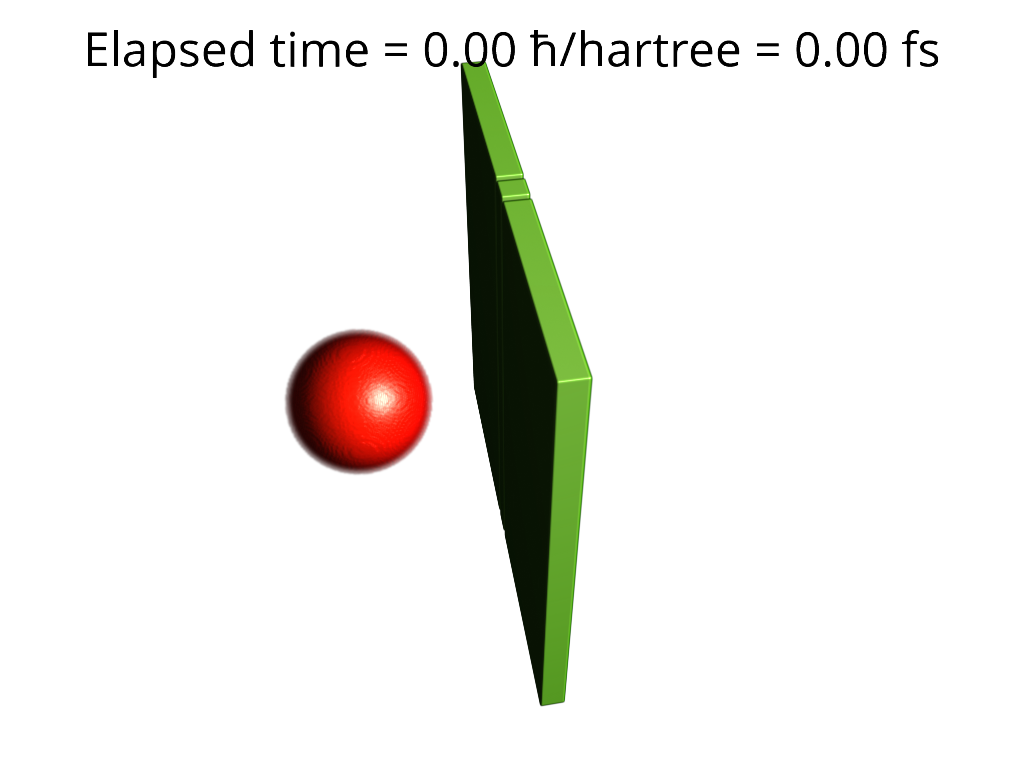
\includegraphics[width=0.45\textwidth]{figures/double_slit_01.png}
		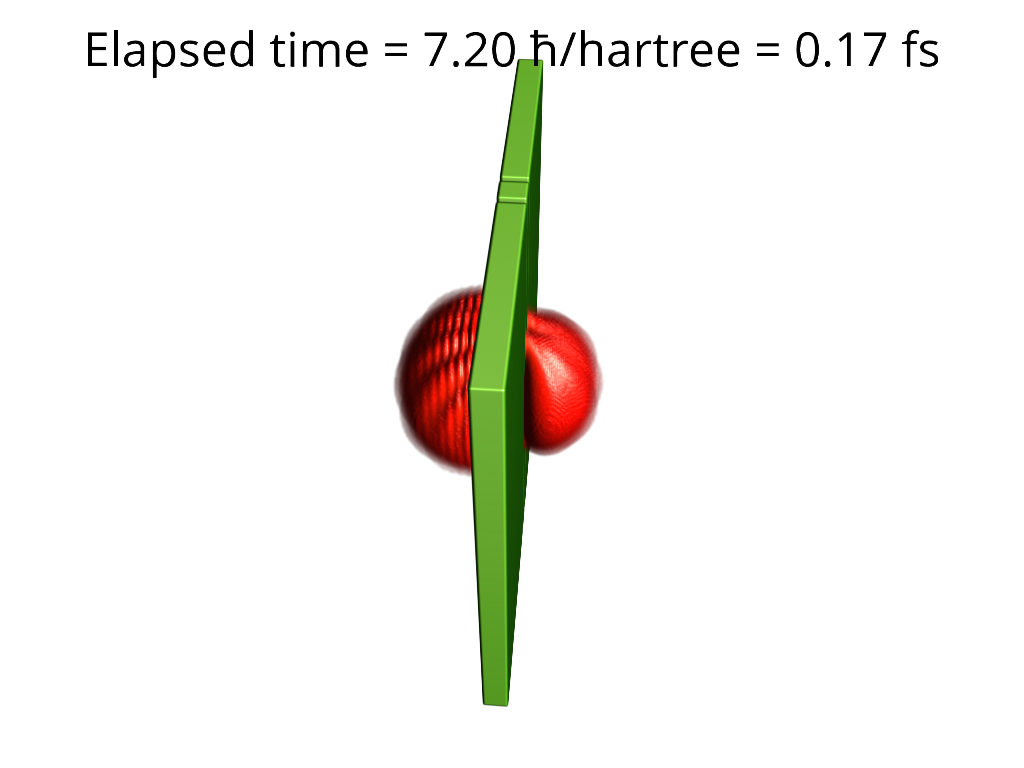
\includegraphics[width=0.45\textwidth]{figures/double_slit_02.png}
		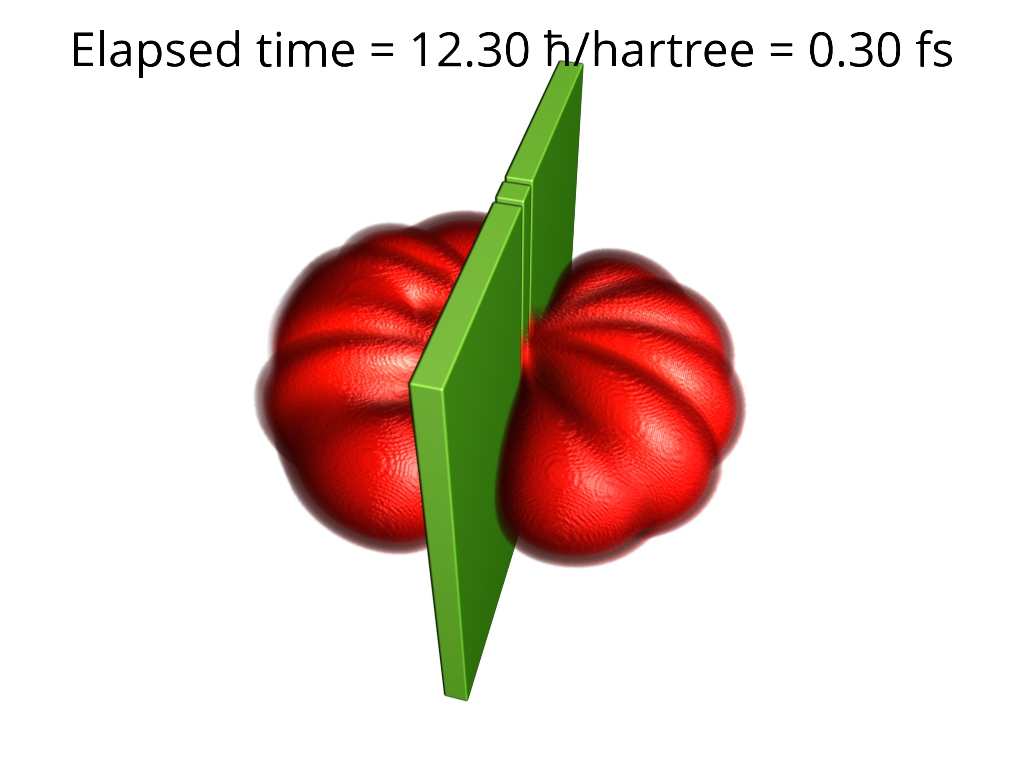
\includegraphics[width=0.45\textwidth]{figures/double_slit_03.png}
		\caption{Stages of the double-slit experiment: before, during, and after passing through the double-slit}
		\label{fig:double_slit_stages}
	\end{center}
\end{figure}
Different stages of double-slit simulation can be seen in figure \ref{fig:double_slit_stages}, where we have used ray tracing to visualize the probability density and the potential.
The interference pattern is visualized in figure \ref{fig:double_slit_interference} on a canvas of size $60 \times 60$ Bohr radius.
We compared the simulated pattern and the pattern predicted by the Huygens–Fresnel principle.
It can be seen that the two patterns are very similar.
The animation of this simulation can be accessed on \url{https://www.youtube.com/watch?v=16M21MPFea0}.
\begin{figure}[hbt!]
	\begin{center}
		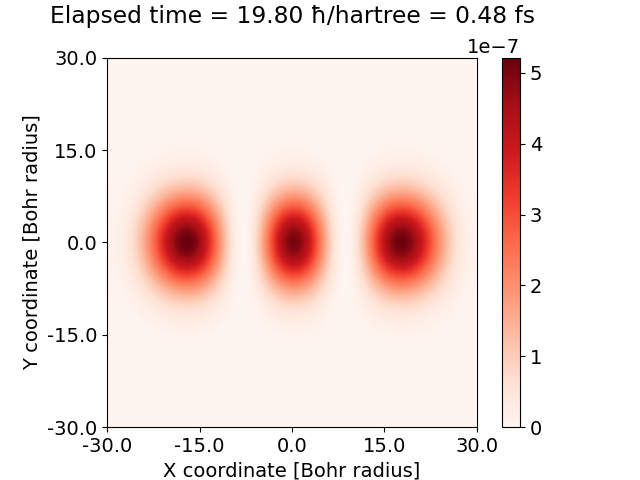
\includegraphics[width=0.6\textwidth]{figures/double_slit_interference.png}
		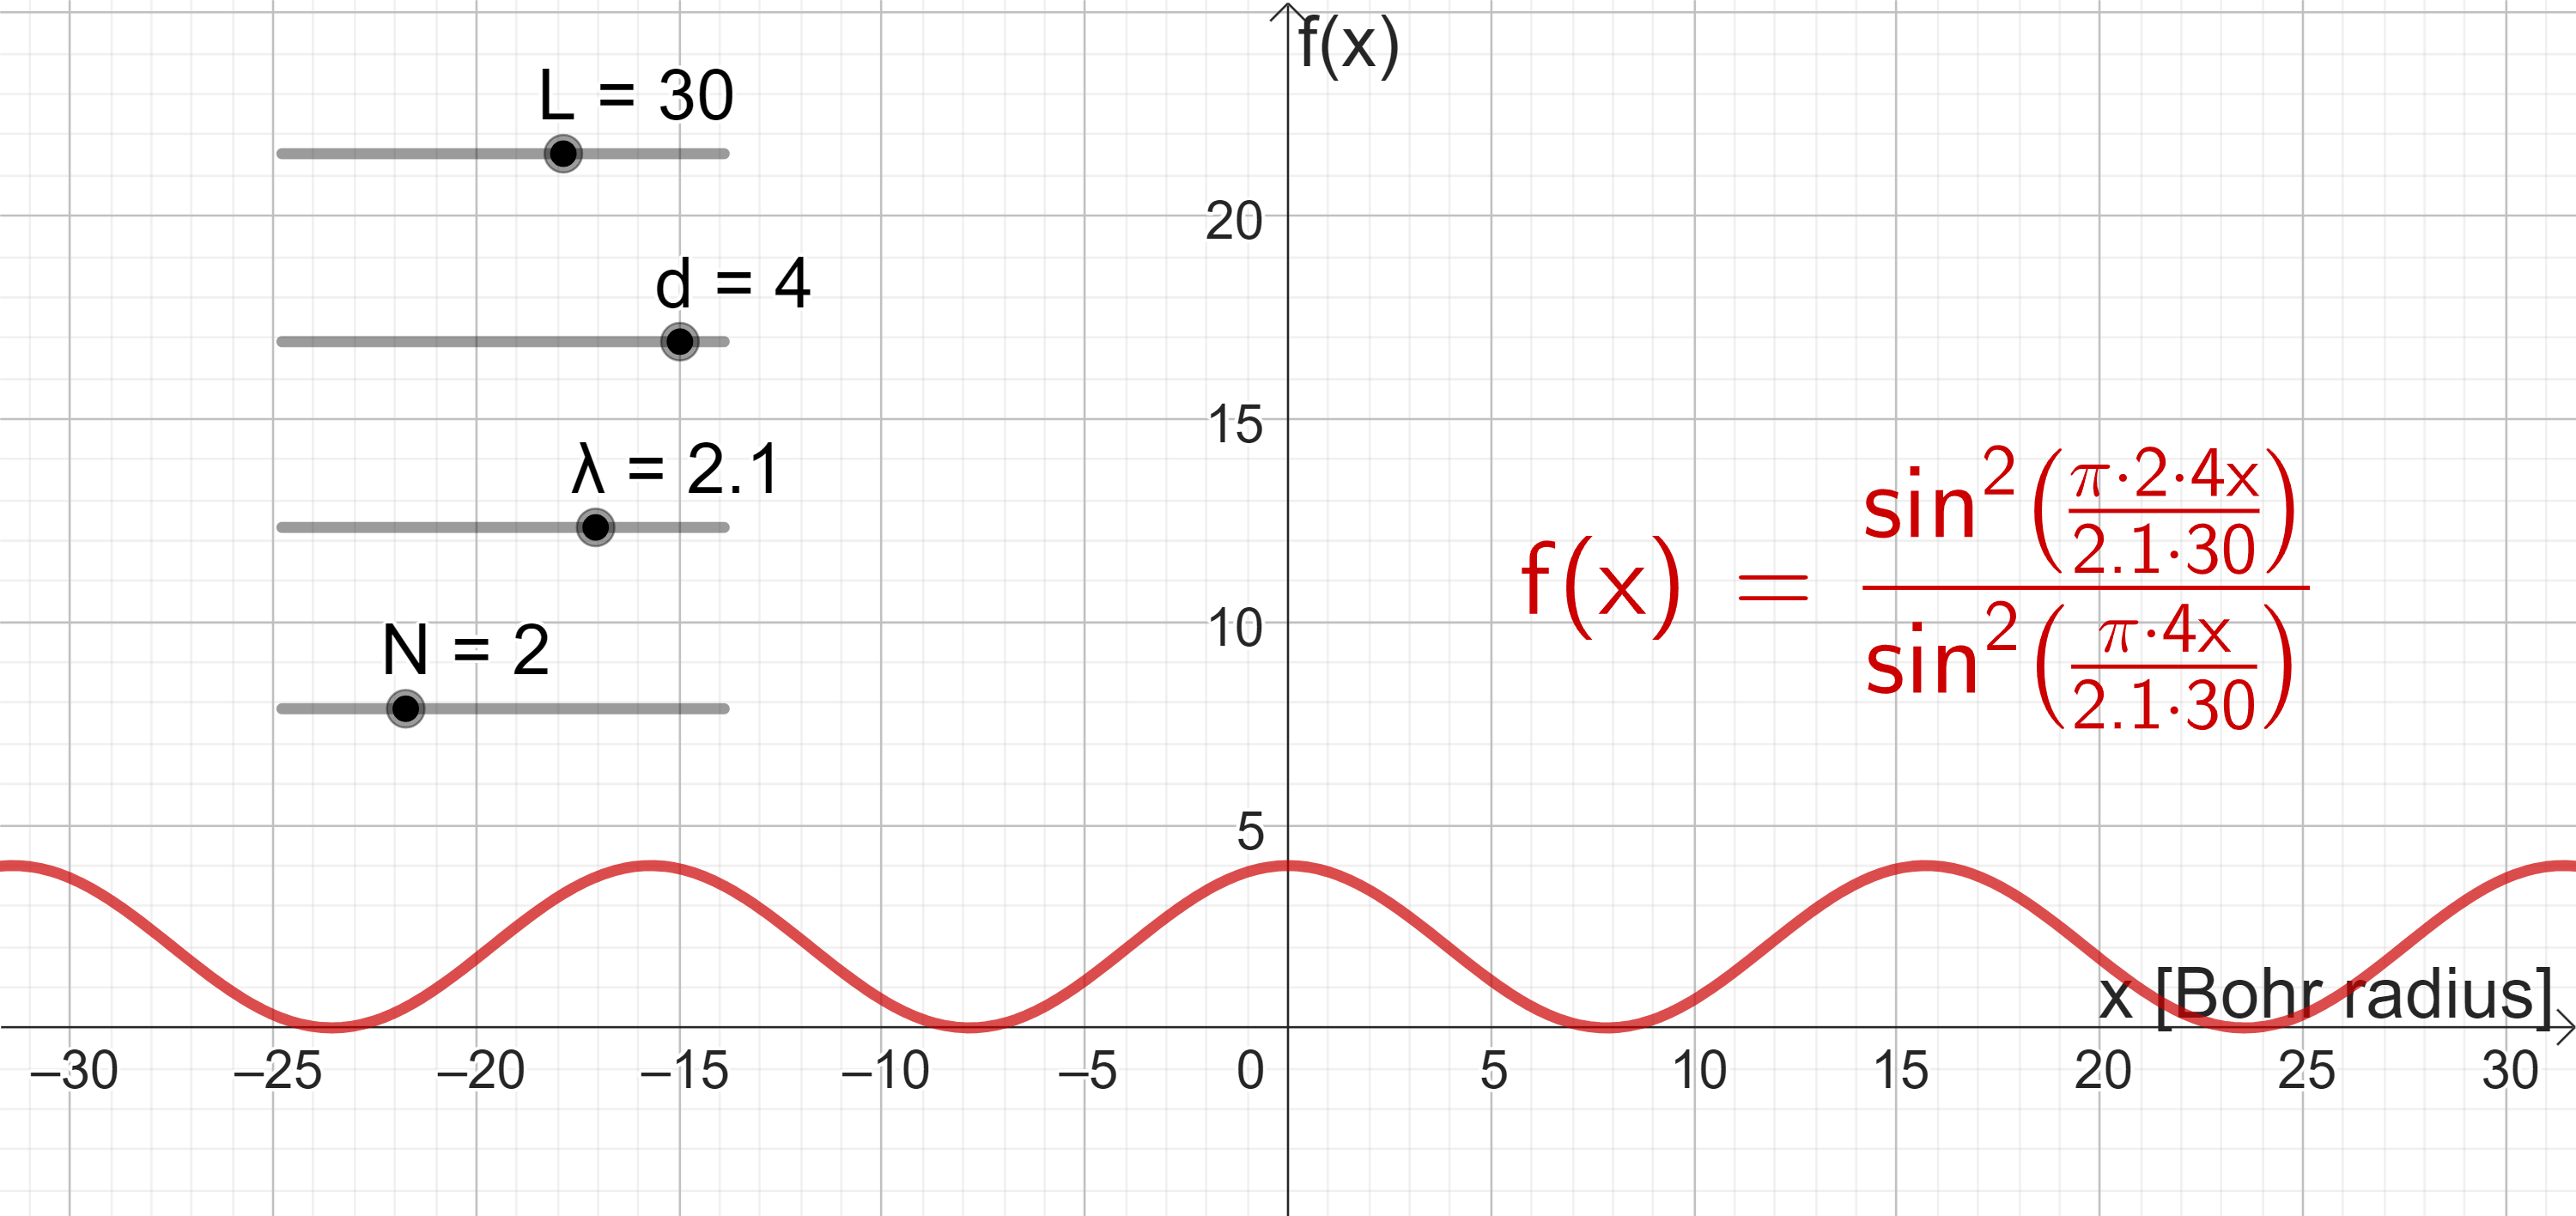
\includegraphics[width=0.6\textwidth]{figures/validation_of_double_slit.png}
		\caption{Comparison of the simulated (above) and the analytically predicted (below) interference pattern during double-slit experiment}
		\label{fig:double_slit_interference}
	\end{center}
\end{figure}

\subsection{Diffraction by optical grating-like potential}

Many different forms of diffraction can be explained using \acrshort{qm}.
The scale at which diffraction happens ranges from the scale of subatomic particles to larger molecules.
Measuring diffraction patterns is a handy tool in the hands of scientists.
It provides information about the object that caused the diffraction.
At this point, it is essential to emphasize that the diffraction of light is a different phenomenon from the diffraction of matter waves since light is an electromagnetic wave.
With that said, the fact that particles are not electromagnetic waves but still exhibit wave-like behavior, as discussed in Section \ref{sec:theory} makes this experiment even more interesting.
Note that in equation \ref{eq:Huygens}, the $y$ is a one-dimensional coordinate. Indeed, the double-slit experiment can be fully described using only two spatial dimensions, and the diffraction pattern forms in a single dimension perpendicular to the propagation direction of the wave.
This is because the localized potential in this scenario is independent of the $z$ coordinate.
To make use of all three simulated dimensions, we also modeled diffraction on diffraction gratings.
In optics, a diffraction grating is a periodic 2D structure that diffracts light \cite{Stroke1967}.
In \acrshort{qm}, such gratings can also be utilized to diffract wave packets.
The holes between the potential nodes behave like the holes in the double-slit experiment.
We put 11 nodes in each direction, forming a rectangular grid.
We experimented with various lattice constants (distance between adjacent grid points).
Here, we present two simulations.
In the first simulation, each node has a Gaussian potential distribution and a maximal potential of $V_{max} = 8$ hartree.
The distance between adjacent grid points is $d = 4$ Bohr radii.
In the second simulation, each node has a Gaussian potential distribution and a maximal potential of $V_{max} = 25$ hartree.
The distance between adjacent grid points is $d = 8$ Bohr radii.
The canvas distance is $L=30$ Bohr radii, and the wavelength of the \acrshort{wp} is $\lambda\simeq 2.1$ Bohr radii for both simulations.
Note in both cases the kinetic energy of the \acrshort{wp} $E = \frac{p^2}{2m} = \frac{h^2}{2\lambda^2} \simeq 4.5$ hartree is less than $V_{max}$.
Otherwise, the grating would not impact the propagation of the \acrshort{wp} sufficiently.
In figure \ref{fig:optical_grid_stages}, we visualized different stages of the time development of the first simulation, and \ref{fig:optical_grid_stages_8_bohr_radii} showcases stages of the second simulation.
Both sequences of rendered images make use of the ray tracing visualization method.
\begin{figure}[hbt!]
	\begin{center}
		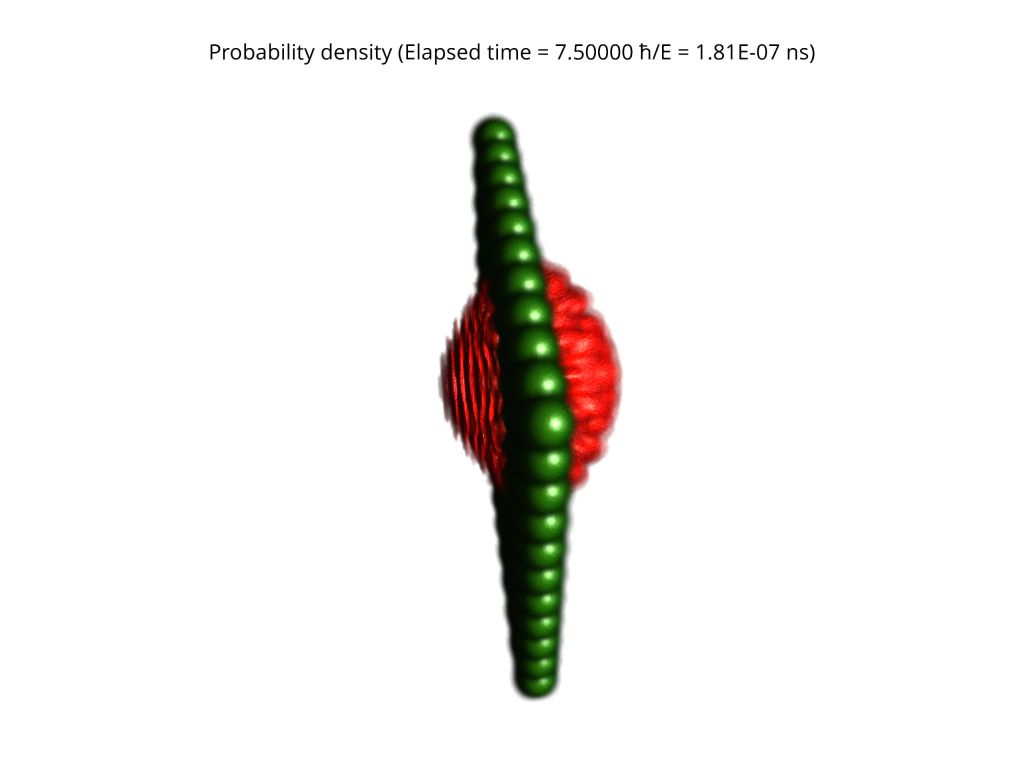
\includegraphics[width=0.45\textwidth]{figures/optical_grid_01.png}
		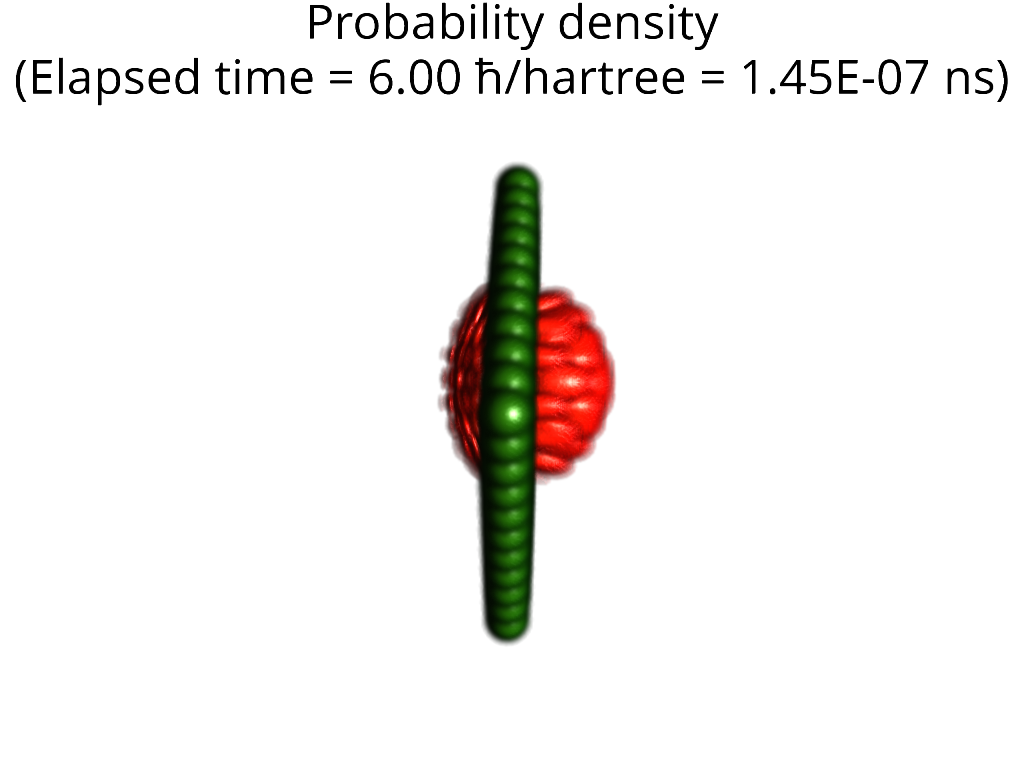
\includegraphics[width=0.45\textwidth]{figures/optical_grid_02.png}
		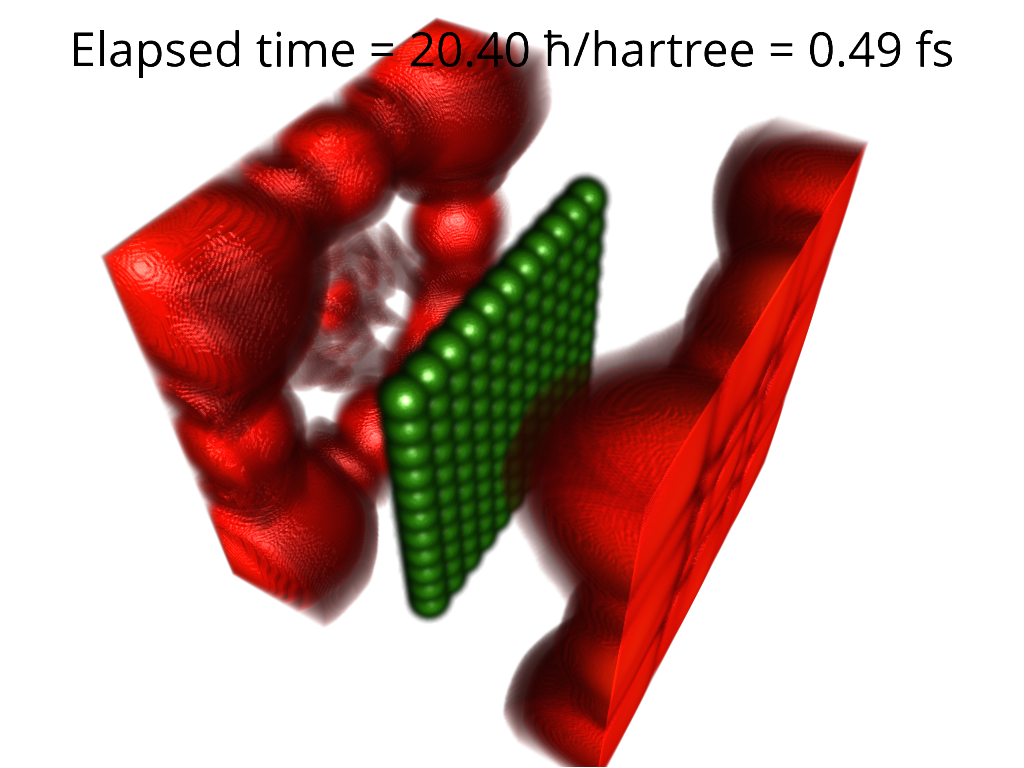
\includegraphics[width=0.45\textwidth]{figures/optical_grid_03.png}
		\caption{Stages of the diffraction grating experiment using a grating with lattice constants of $4$ Bohr radii: during, right after, and later after passing through the grating}
		\label{fig:optical_grid_stages}
	\end{center}	
\end{figure}
\begin{figure}[hbt!]
	\begin{center}
		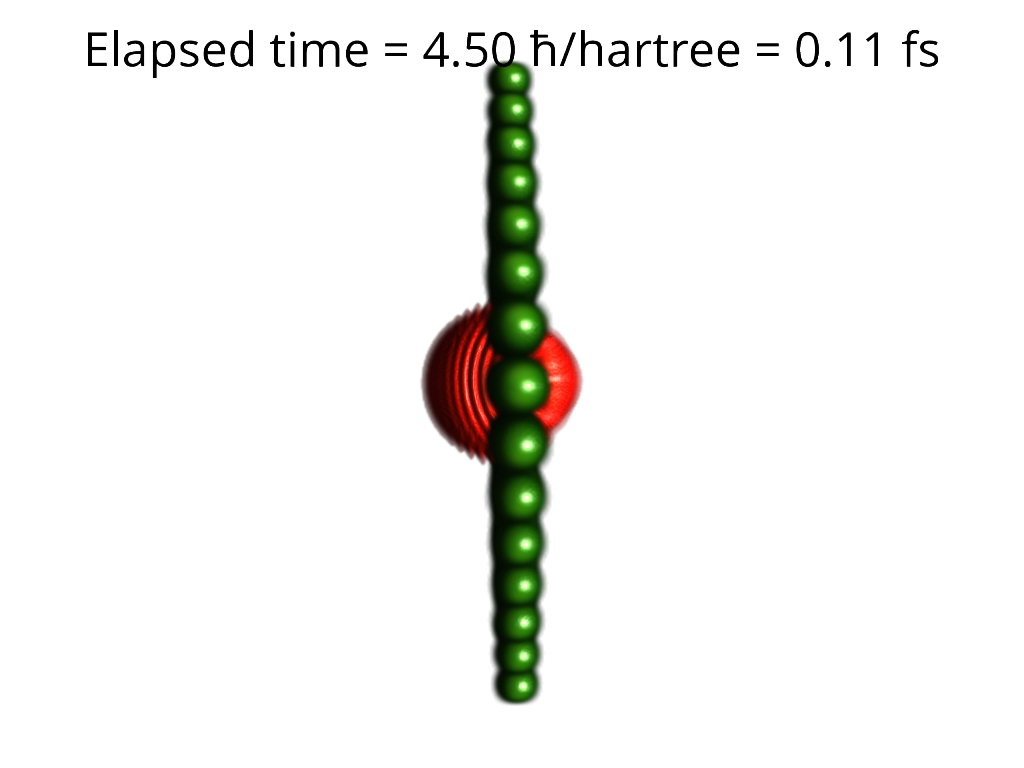
\includegraphics[width=0.45\textwidth]{figures/optical_grid_8_bohr_rad_01.png}
		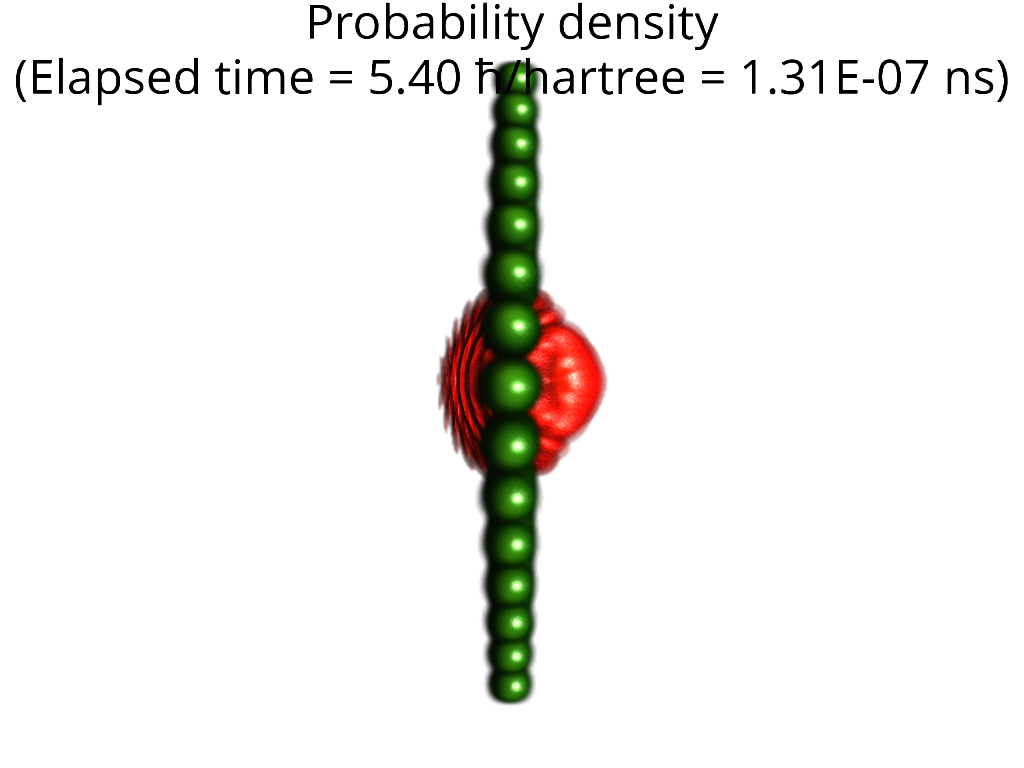
\includegraphics[width=0.45\textwidth]{figures/optical_grid_8_bohr_rad_02.png}
		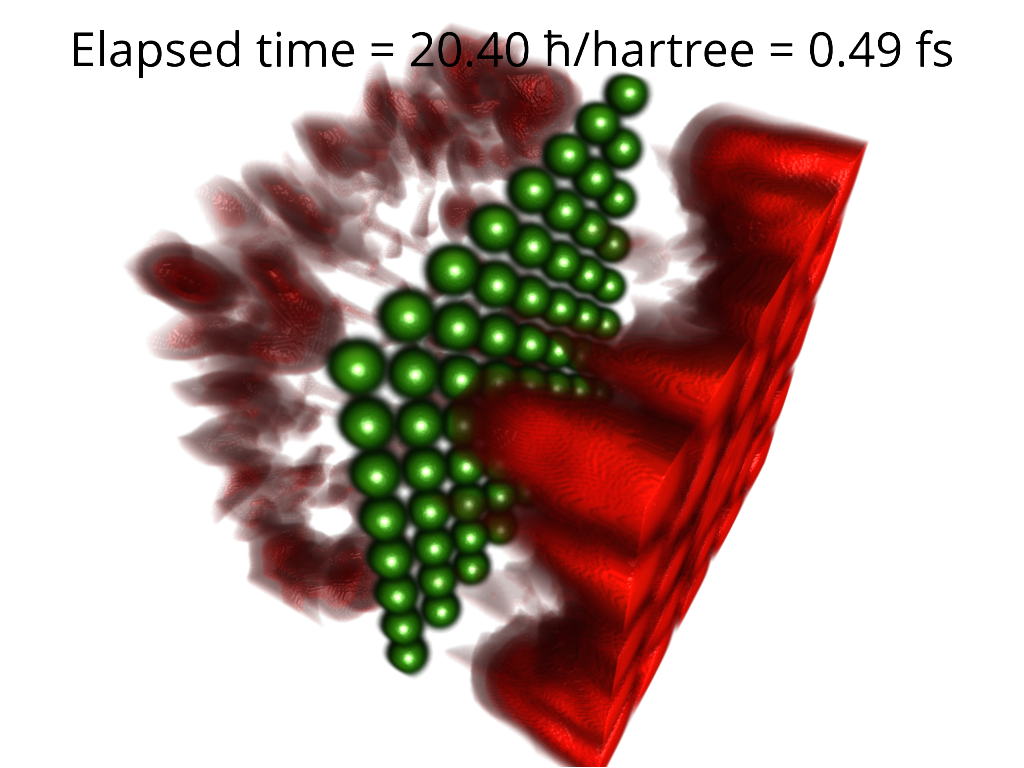
\includegraphics[width=0.45\textwidth]{figures/optical_grid_8_bohr_rad_03.png}
		\caption{Stages of the diffraction grating experiment using a grating with lattice constants of $8$ Bohr radii: during, right after, and later after passing through the grating}
		\label{fig:optical_grid_stages_8_bohr_radii}
	\end{center}	
\end{figure}

During the simulation, many interesting interference patterns arise.
We showcase some of these for the $4$ Bohr radius lattice constant case in figure \ref{fig:optical_grid_interference} and for the $8$ Bohr radius lattice constant case in figure \ref{fig:optical_grid_interference_8_grid}.
The animations showing the results in motion can be found on \url{https://youtu.be/KCE5xqm-diQ?si=-kzjWvaw8zOcAz4C} and \url{https://youtu.be/YCadOpsx9y8}.
\begin{figure}[hbt!]
	\begin{center}
		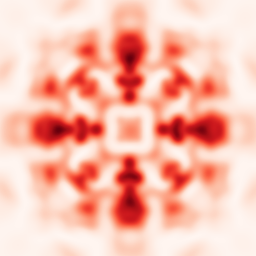
\includegraphics[width=0.49\textwidth]{figures/optical_grid_interference_01.png}
		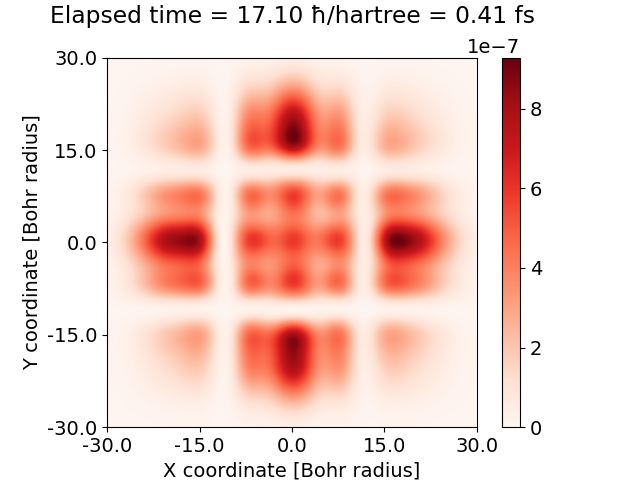
\includegraphics[width=0.49\textwidth]{figures/optical_grid_interference_02.png}
		\caption{Two stages of interference patterns forming on the measurement canvas during diffraction grating simulation using lattice constant of $4$ Bohr radii}
		\label{fig:optical_grid_interference}
	\end{center}	
\end{figure}
\begin{figure}[hbt!]
	\begin{center}
		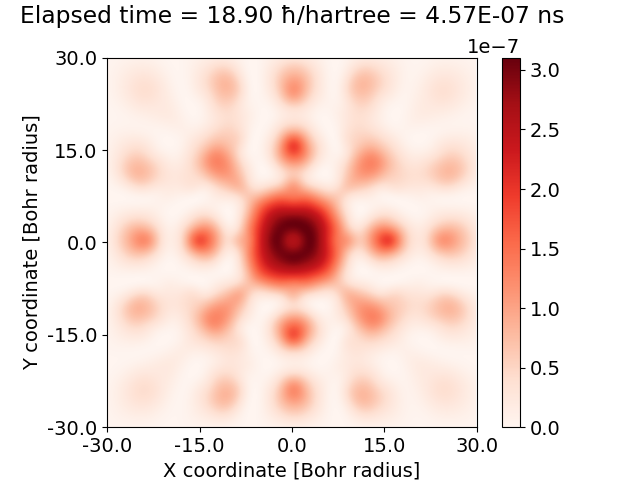
\includegraphics[width=0.49\textwidth]{figures/optical_grid_interference_01_8_grid.png}
		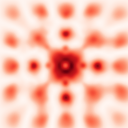
\includegraphics[width=0.49\textwidth]{figures/optical_grid_interference_02_8_grid.png}
		\caption{Two stages of interference patterns forming on the measurement canvas during diffraction grating simulation using lattice constant of $8$ Bohr radii}
		\label{fig:optical_grid_interference_8_grid}
	\end{center}	
\end{figure}

\subsection{Many-body interactions}

One interesting use case of a higher dimensional \acrshort{wpd} simulator is that the higher dimensional space can be used to model the interactions between multiple lower-dimensional particles.
For example, our 3D simulation is capable of the simulation of three 1D particles.
To do this, we have to define special interaction potential.
To create such potential, we have to think about the coordinates in the higher dimensional configuration space as the coordinates of the lower dimensional space describing the location of the lower dimensional particle.
If the potential energy affecting all particles can be expressed as a $V(x_a, x_b, x_c)$ function of the location of particle $A$ and $B$ and $C$, then we can reinterpret this function as the $V(\vec{r})$ localized potential function used in the potential propagator in equation \ref{eq:potential_prop}.
Note that here $\vec{r}$ becomes $(x_a, x_b, x_c)$.
To model the interaction between the three 1D particles, we initialized a linear combination of two types of interaction potentials.
One is proportional to $\frac{1}{|x_i - x_j|}$ where $i,j\in\{a,b,c\}$ and $i\neq j$ and the other is a hard interaction that takes its maximum if the particles approach each other inside an $\epsilon$ radius otherwise it is zero.
To prevent blotting of the Gaussian \acrshort{wp} we also initialized a harmonic oscillator potential.
This helps because the Gaussian \acrshort{wp} is the eigenstate of the harmonic oscillator.
The potential for a harmonic oscillator is given in the following form
\begin{equation}
	\label{eq:harmonic_osc}
	V(x) = \frac{m\omega^2}{2}x^2
\end{equation}
where $m$ is the oscillating mass and $\omega$ is the angular frequency of the oscillation.
Our first simulation of 1D particles is somewhat similar to the classical Newton's cradle \cite{Gauld2006}
in the sense that it demonstrates momentum transfer between multiple particles.
We created a scenario where particle $A$ starts at $25$ Bohr radii away from the center of the oscillator where the potential energy is maximal; thus, it accelerates towards the other two particles ($B$ and $C$), consequently transferring the momentum to particle $C$ on the far right.
For this experiment, the interaction potential consists only of the hard interaction.
The angular frequency of the oscillator was selected to be $\omega = \frac{2\pi}{40} \simeq 0.1571\; \frac{rad\cdot hartree}{\hbar}$.
After the momentum transfer, particle $C$ propagates towards the maximal potential of the oscillator on the far right.
Particle $B$ stays in place since it serves only as a medium in the momentum transfer.
The momentum gained from particle $A$ was immediately given to particle $C$.
When all the kinetic energy of the moving particle is transferred to potential energy, then it turns back.
The oscillation with the momentum transfer between the particles continues.
Different phases of this simulation can be observed on the per-axis visualization in figure \ref{fig:1d_particles_in_oscillator_stages}.
The corresponding animation can be found on \url{https://youtu.be/zOiYACVOssU}.
\begin{figure}[hbt!]
	\begin{center}
		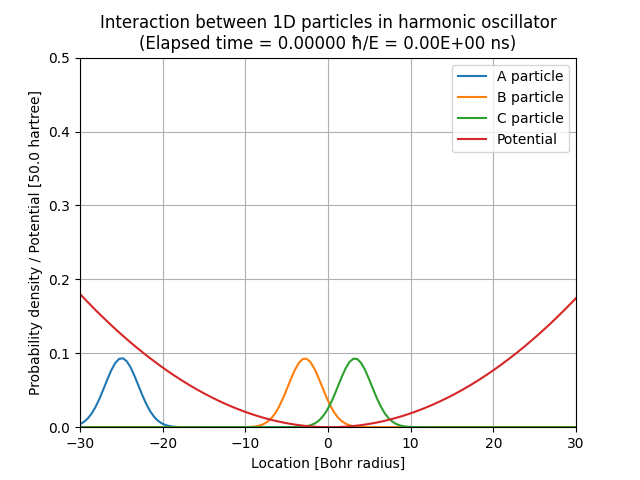
\includegraphics[width=0.45\textwidth]{figures/1d_oscillator_01.png}
		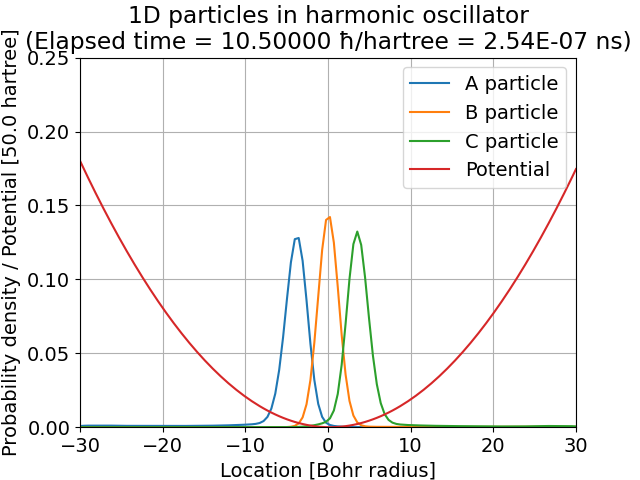
\includegraphics[width=0.45\textwidth]{figures/1d_oscillator_02.png}
		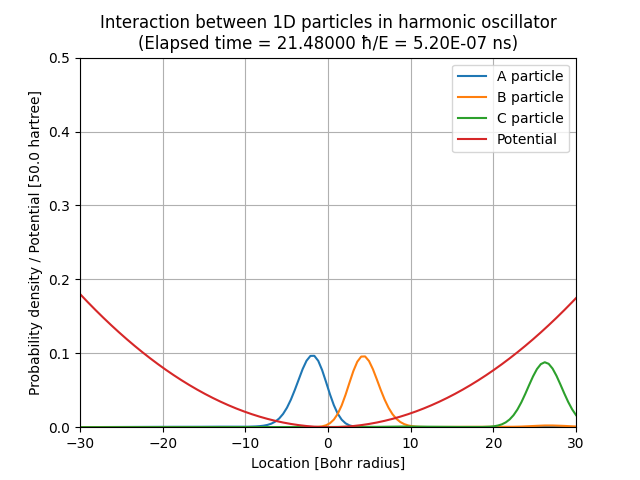
\includegraphics[width=0.45\textwidth]{figures/1d_oscillator_03.png}
		\caption{Stages of the interactions between 1D particles in harmonic oscillator: initial state, particle A giving momentum to particle C, particle C reaching maximal potential and turning back}
		\label{fig:1d_particles_in_oscillator_stages}
	\end{center}
\end{figure}
Please note that particle $C$ converts all of its kinetic energy to potential energy right at the half of the first period of the oscillation $t = 40 / 2 \frac{\hbar}{hartree} = 20 \frac{\hbar}{hartree}$.
This means that the harmonic oscillator functions correctly.

Now, let us repeat this experiment, but now we place a finite potential barrier in the middle of the oscillator.
In Tamás Geszti's book \cite{geszti2007}, we can find that the probability of a particle with $E$ energy tunneling through a $d$ thick barrier of $V_0$ potential can be expressed in the following form
\begin{equation}
	\label{eq:tunneling_probability}
	\probP_{tunnel} = \frac{1}{1 + \frac{V_0^2}{4E(V_0 - E)}sinh^2(\kappa d)}
\end{equation}
where $\kappa = \sqrt{2m(V_0 - E)}\;/\hbar$ is determined by the energy of the incoming \acrshort{wp}.
Energy is conserved, so $E = V(x_A)$.
We solve for $\probP_{tunnel} = \frac{1}{2}$.
One possible solution is $V_0 \simeq 9.8$ hartree and $d \simeq 0.3$ Bohr radius.
Particle $A$ gives its momentum to $B$ as before.
With these parameters, approximately half of the probability density of particle $B$ tunnels through the barrier, giving its momentum to particle $B$ on the next side of the wall.
This causes the $C$ to start moving with a probability of approximately $\frac{1}{2}$.
What we just described is called the entanglement of the states of particles $A$, $B$, and $C$.
Let's perform a measurement to determine the location of particles $A$, $B$, and $C$ shortly after the first momentum transfer could have happened.
If we would measure particle $A$ to be located in the middle of the harmonic oscillator, that means that it gave its momentum to particle $B$ and $B$ has tunneled through the finite potential barrier.
If $B$ tunneled, that also means that beyond the barrier, it collided with particle $C$, consequently transferring all its kinetic energy to $C$.
On the contrary, if the result of the measurement determining the location of particle $A$ would have shown that particle $A$ bounced back from $B$, that means that $B$ did not tunnel through the barrier.
This also means that particle $C$ did not receive any kinetic energy and stayed stationary right beyond the barrier.
The measurement of the state of one entangled particle determines the outcome of the measurement of the other entangled particles.
Real-life experiments are sound with this thought experiment \cite{Vasilyev2017}.
The probability density plot can be observed in figure \ref{fig:1d_osc_with_tunneling}.
The animation of this simulation can be found on \url{https://youtu.be/IVb_mpzmuYA}.
\begin{figure}[hbt!]
	\begin{center}
		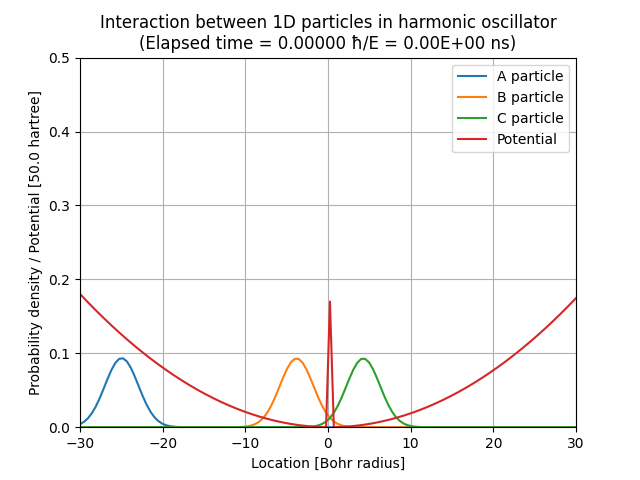
\includegraphics[width=0.45\textwidth]{figures/1d_oscillator_tunneling_01.png}
		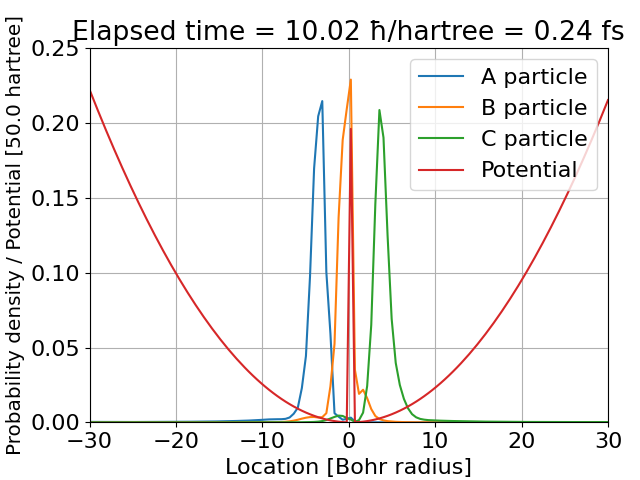
\includegraphics[width=0.45\textwidth]{figures/1d_oscillator_tunneling_02.png}
		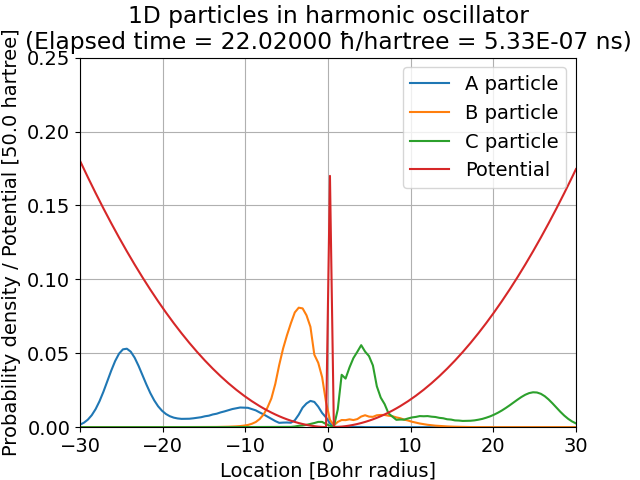
\includegraphics[width=0.45\textwidth]{figures/1d_oscillator_tunneling_03.png}
		\caption{Stages of the interactions between 1D particles in harmonic oscillator with finite potential barrier: initial state, particle A giving momentum to particle C with approximately 0.5 probability, particle C reaching maximal potential and turning back with approximately 0.5 probability}
		\label{fig:1d_osc_with_tunneling}
	\end{center}	
\end{figure}

\subsection{Modeling a flash memory cell}

Our last group of simulations tries to model the working of a flash memory cell.
Flash memory is used extensively in many modern electronic devices such as smartphones, laptops, or tablets.
The general structure of a cell is visualized in figure \ref{fig:flash_memory}.
The structure of a flash memory cell resembles a \acrfull{mosfet} \cite{Korec2011}.
The difference is that the memory cell has two gates: the control gate, which is connected to a control line similarly to regular transistors, and the floating gate, which is insulated from all sides by oxide layers.
Both the control gate and the floating gate are made out of conducting material (metal or polysilicon).
In figure \ref{fig:flash_memory}, it can be seen that between the control gate and the floating gate, there is a thicker potential barrier.
This prevents the flow of electrons between these two parts.
Only the Coulomb potential induced by the electrons on the control gate must be felt by the electrons on the floating gate.
A flash memory cell stores information by trapping electrons on a floating gate.
The reading of a memory cell is done by inducing a current through the channel between the source and drain.
If there are electrons trapped on the floating gate, they create an electric field affecting the substrate.
The substrate is made out of semiconducting material. (Generally silicon.)
A semiconductor changes conductivity based on the electromagnetic field.
If there are electrons on the floating gate, the channel between the source and drain has higher resistance.
By measuring the current through this channel, the information about the state of the floating gate can be retrieved.
This is used to store bits of information.
In our model, we simulate one single cell, and this cell only stores a single bit of information.
We only model one single electron that can be trapped on the floating gate.
The writing and flushing of the flash cell are performed by applying voltage on the control gate, inducing a strong enough electric field that the electron can tunnel through the potential barrier between the floating gate and the channel.
\begin{figure}[hbt!]
	\centering
	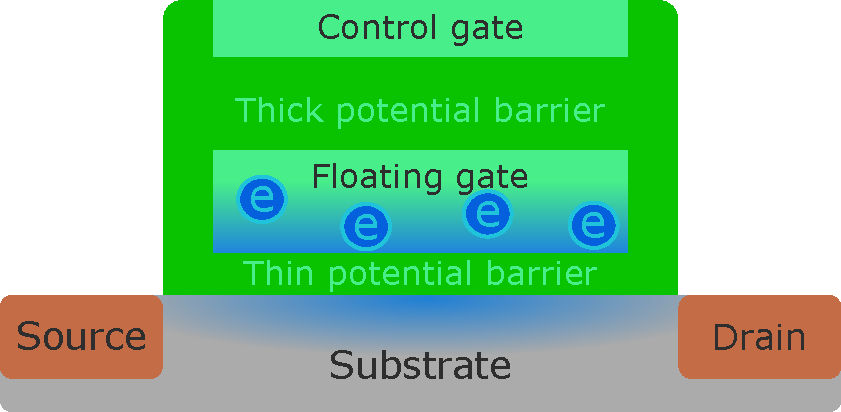
\includegraphics[width=0.5\textwidth]{figures/flash_memory.pdf}
	\caption{Schematic structure of a flash memory cell}
	\label{fig:flash_memory}
\end{figure}
For the writing and flushing to be possible, the thickness and height of the oxide layer --consequently, the potential wall-- between the floating gate and the substrate must be chosen carefully.
This barrier must be thick enough to prevent unwanted tunneling when no voltage is applied to the control gate.
After the control gate fills with electrons, the Coulomb potential created by those electrons makes an overall slope in the potential barrier created by the oxide layer.
The potential level inside the floating gate does not acquire a slope since it is made out of conducting material, hence its equipotential.
This slope is added to the potential barrier, thus changing its shape.
The previously rectangular barrier now acquired a triangular outline. More importantly, the $d$ width of the barrier gets reduced.
This increases the probability of the electron in the floating gate tunneling out from the gate through the thin oxide layer into the substrate.
This phenomenon is called Fowler–Nordheim tunneling \cite{Fowler_1928bv}.
Figure \ref{fig:fowler_nordheim_tunneling} visualizes the principle of this effect.
\begin{figure}[hbt!]
	\centering
	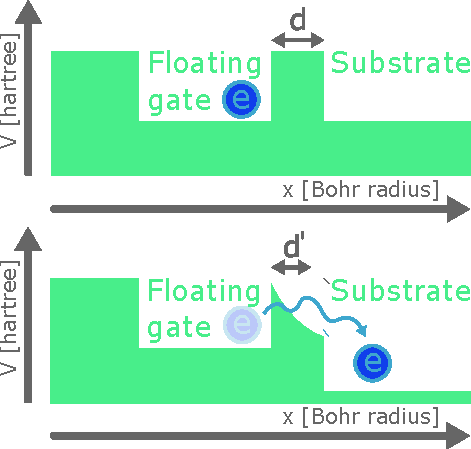
\includegraphics[width=0.5\textwidth]{figures/fowler_nordheim_tunneling.pdf}
	\caption{Fowler-Nordheim tunneling: on the upper image there is no Coulomb potential; on the image below Coulomb potential changes the shape of potential barrier causing tunneling}
	\label{fig:fowler_nordheim_tunneling}
\end{figure}
In our flash memory cell simulation, we initialized a potential wall representing the barrier between the floating gate and the substrate.
Our simulation deals with only one electron.
To simulate the flushing of the gate, we initialize the location of this electron to be inside the floating gate.
We add a Coulomb potential that decreases inside the thin oxide layer towards the substrate.
We initialized the barrier with a height of $V_0 = 10$ hartree and width of $d = 4.0$ Bohr radius.
We surrounded the floating gate area with thick potential barriers from the remaining five sides to prevent tunneling in unwanted directions. However, we excluded these from the visualization to make the electron's probability density visible from the outside.
We model the charge on the control gate as a uniformly charged infinite sheet.
This way, the Coulomb potential induced by a negatively charged control gate acting on an electron inside the oxide can be described by the following formula
\begin{equation}
	\label{eq:coulomb_potential}
	V_C = \frac{\sigma}{2r\epsilon}
\end{equation}
where $\epsilon$ is the dielectric permittivity of the oxide, $\sigma$ is the surface charge density at the control gate, and $r$ is the distance from the control gate.
Inside the floating gate, the potential stays zero.
On the thin oxide layer between the floating gate and the substrate, the slope of the potential has to be significant enough so that the probability of tunneling increases.
We initialized the Coulomb potential to create a steep enough slope at the start of the oxide.
For this, we set the charge density to $600 \frac{elementary charge}{(Bohr radius)^2}$ and the thickness of the oxide between the control gate and the floating gate to $10$ Bohr radius.
This is significant because although the gate is on equipotential, right after the gate, the Coulomb potential continues to decrease.
For simplicity, we choose $\epsilon$ to be equal to one.
With this setup the derivative of potential at the start of the oxide is $V' = \frac{d}{dr}\frac{\sigma}{2r\epsilon} = -\frac{\sigma}{2r^2\epsilon} = -\frac{600}{2\cdot 10^2\cdot 1} = 3\; \frac{\text{hartree}}{\text{Bohr radius}}$.
The potential barrier between the floating gate and the substrate was chosen to be $1$ Bohr radius thick and $8$ hartree high.
An electron inside the floating gate would have some kinetic energy, so we gave it an initial momentum of $3\; \frac{\hbar}{\text{Bohr radius}}$.
We ran the simulation with the Coulomb potential turned on and off and compared the \textit{probability evolution} plots.
Figure \ref{fig:flash_flush_plot} shows the flushing of the floating gate with the Coulomb potential enabled.
The probability of the electron being found on the floating gate is decreasing.
The step-like nature of the plot is caused by the bouncing of the wave packet inside the gate.
Also, note that the probability of the particle being found inside full volume is decreasing.
This is because we left the underside of the substrate open to prevent unwanted reflections from that barrier.
In that direction, the tunneling particle can leave the substrate freely.
In our simulation, the parts of the \acrshort{wp} leaving the visualized area get absorbed by the draining potential.
At first glance, the rate at which the particle leaves the gate seems slow.
Bear in mind that we are working with atomic units.
Figure \ref{fig:flash_flush_plot} shows that after $40\;\frac{\hbar}{\text{hartree}} \simeq 0.96 \text{femtoseconds}$ the probability of the particle located on the gate decreased by $10\%$.
\begin{figure}[hbt!]
	\centering
	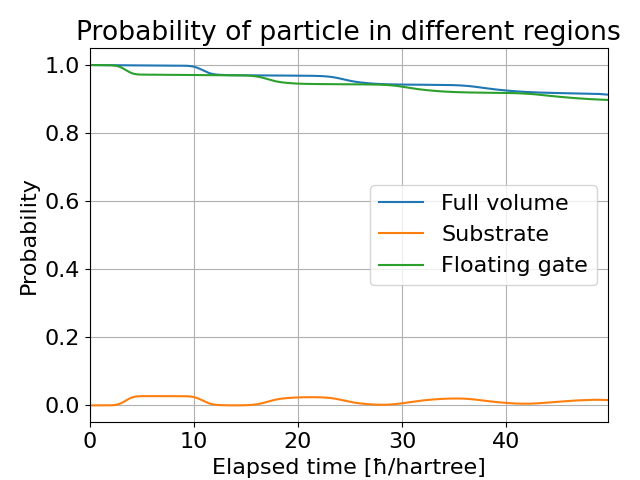
\includegraphics[width=0.5\textwidth]{figures/flash_flush.png}
	\caption{Flushing of the floating gate: the probability of the particle being found on the floating gate is gradually decreasing}
	\label{fig:flash_flush_plot}
\end{figure}
In figure \ref{fig:flash_keep}, however, the electron stays on the gate since we disabled the Coulomb potential.
\begin{figure}[hbt!]
	\centering
	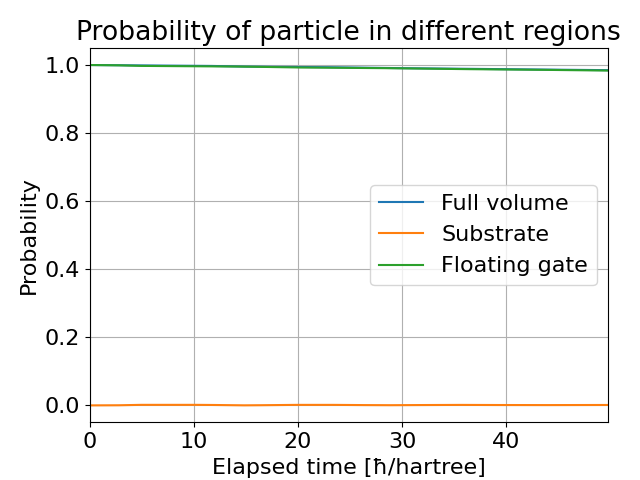
\includegraphics[width=0.5\textwidth]{figures/flash_keep.png}
	\caption{Storing the electron on the floating gate: there is no Fowler-Nordheim tunneling}
	\label{fig:flash_keep}
\end{figure}
For the flushing of the gate, we also provide ray-traced visualization of the flash memory cell simulation.
This can be observed in figure \ref{fig:flash_memory_ray_traced} and in animated form on \url{https://youtu.be/0-FTkSJgPPs?si=sl5k4ubo8XstPJ1b}.
In these images, we only visualize the potential barrier between the control gate and floating gate (top green layer), the single electron trapped inside the floating gate (with red), and the potential barrier between the floating gate and substrate (lower green layer).
The simulation also incorporates the remaining walls around the floating gate and the Coulomb potential.

\begin{figure}[hbt!]
	\begin{center}
		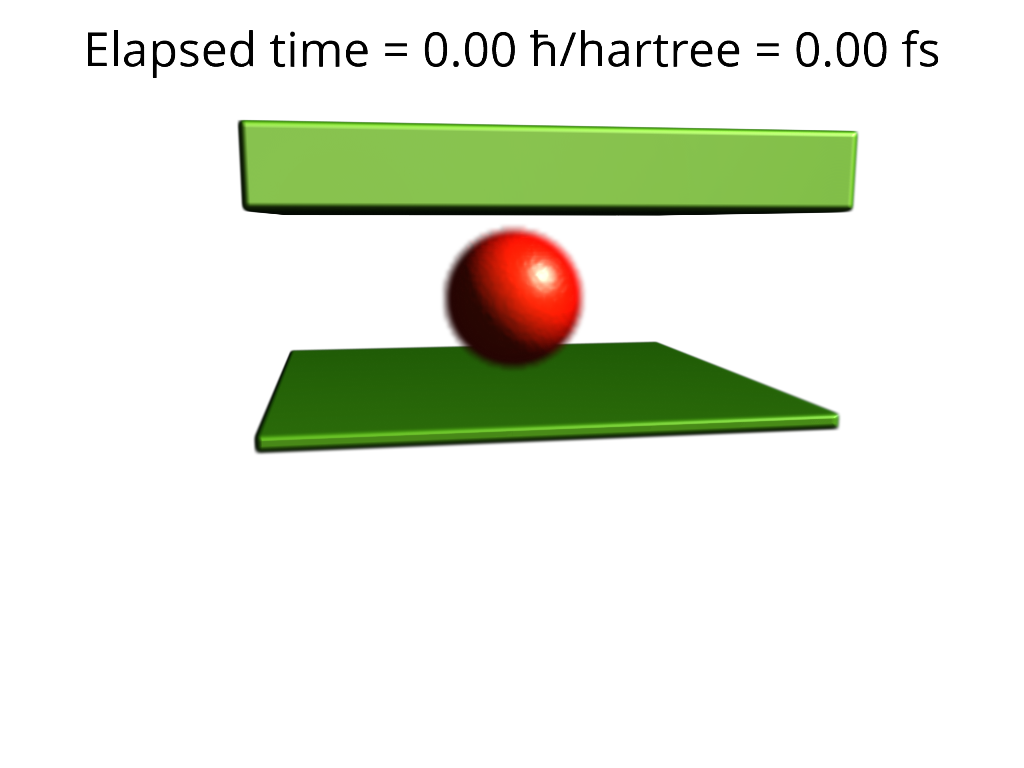
\includegraphics[width=0.45\textwidth]{figures/flash_memory_01.png}
		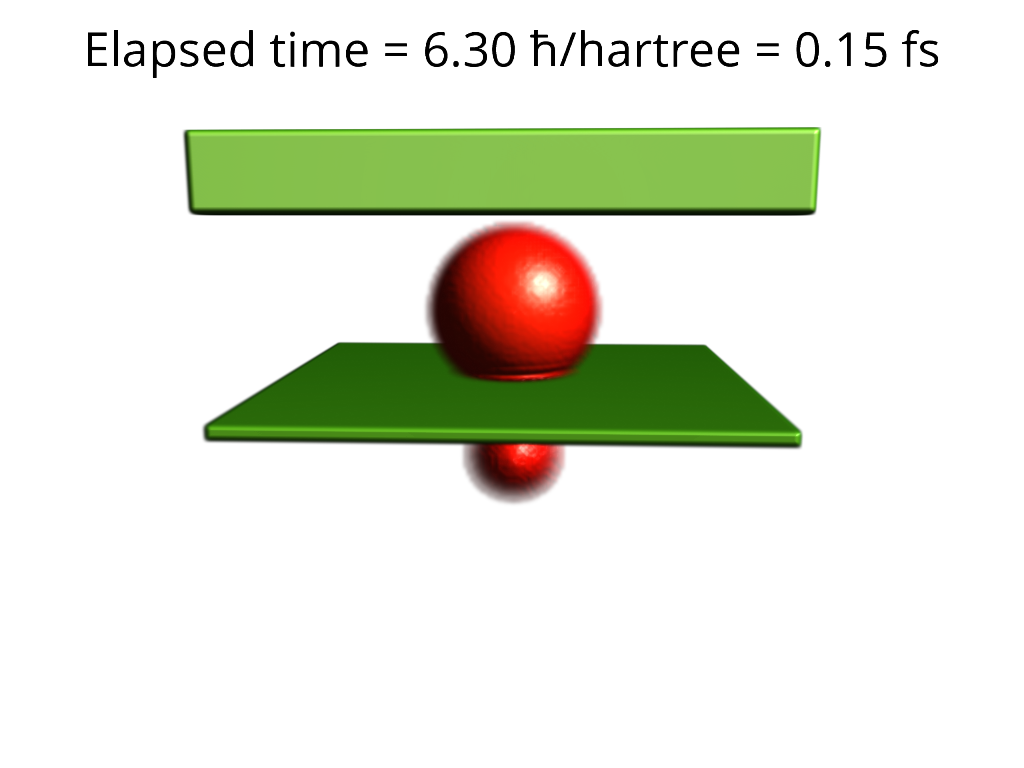
\includegraphics[width=0.45\textwidth]{figures/flash_memory_02.png}
		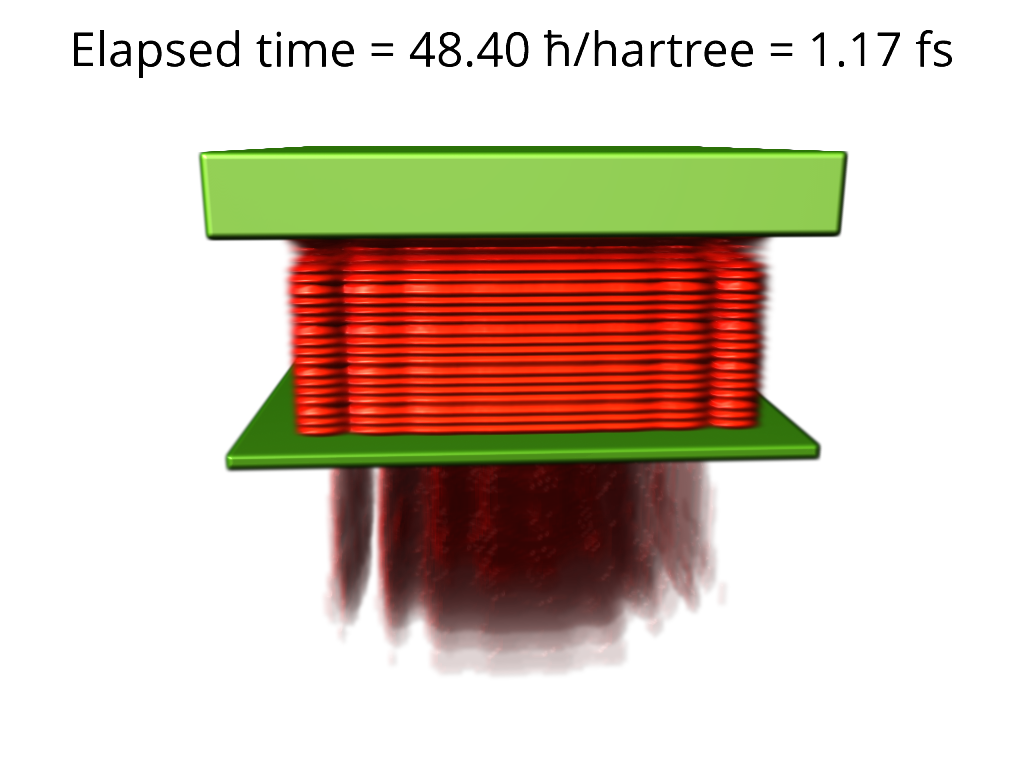
\includegraphics[width=0.45\textwidth]{figures/flash_memory_03.png}
		\caption{Flushing a trapped electron from the floating gate of a flash memory cell: initial state; first tunneling; after multiple bounces inside the gate}
		\label{fig:flash_memory_ray_traced}
	\end{center}
\end{figure}


